

\section{Introduction}

\url{https://helgeklein.com/blog/permissions-a-primer-or-dacl-sacl-owner-sid-and-ace-explained/#dissecting-security-descriptors-sd}

the following
\href{https://docs.microsoft.com/en-us/windows/security/identity-protection/access-control/security-principals}{picture}
diagram illustrates the Windows authorization and access control process.
\begin{figure}
  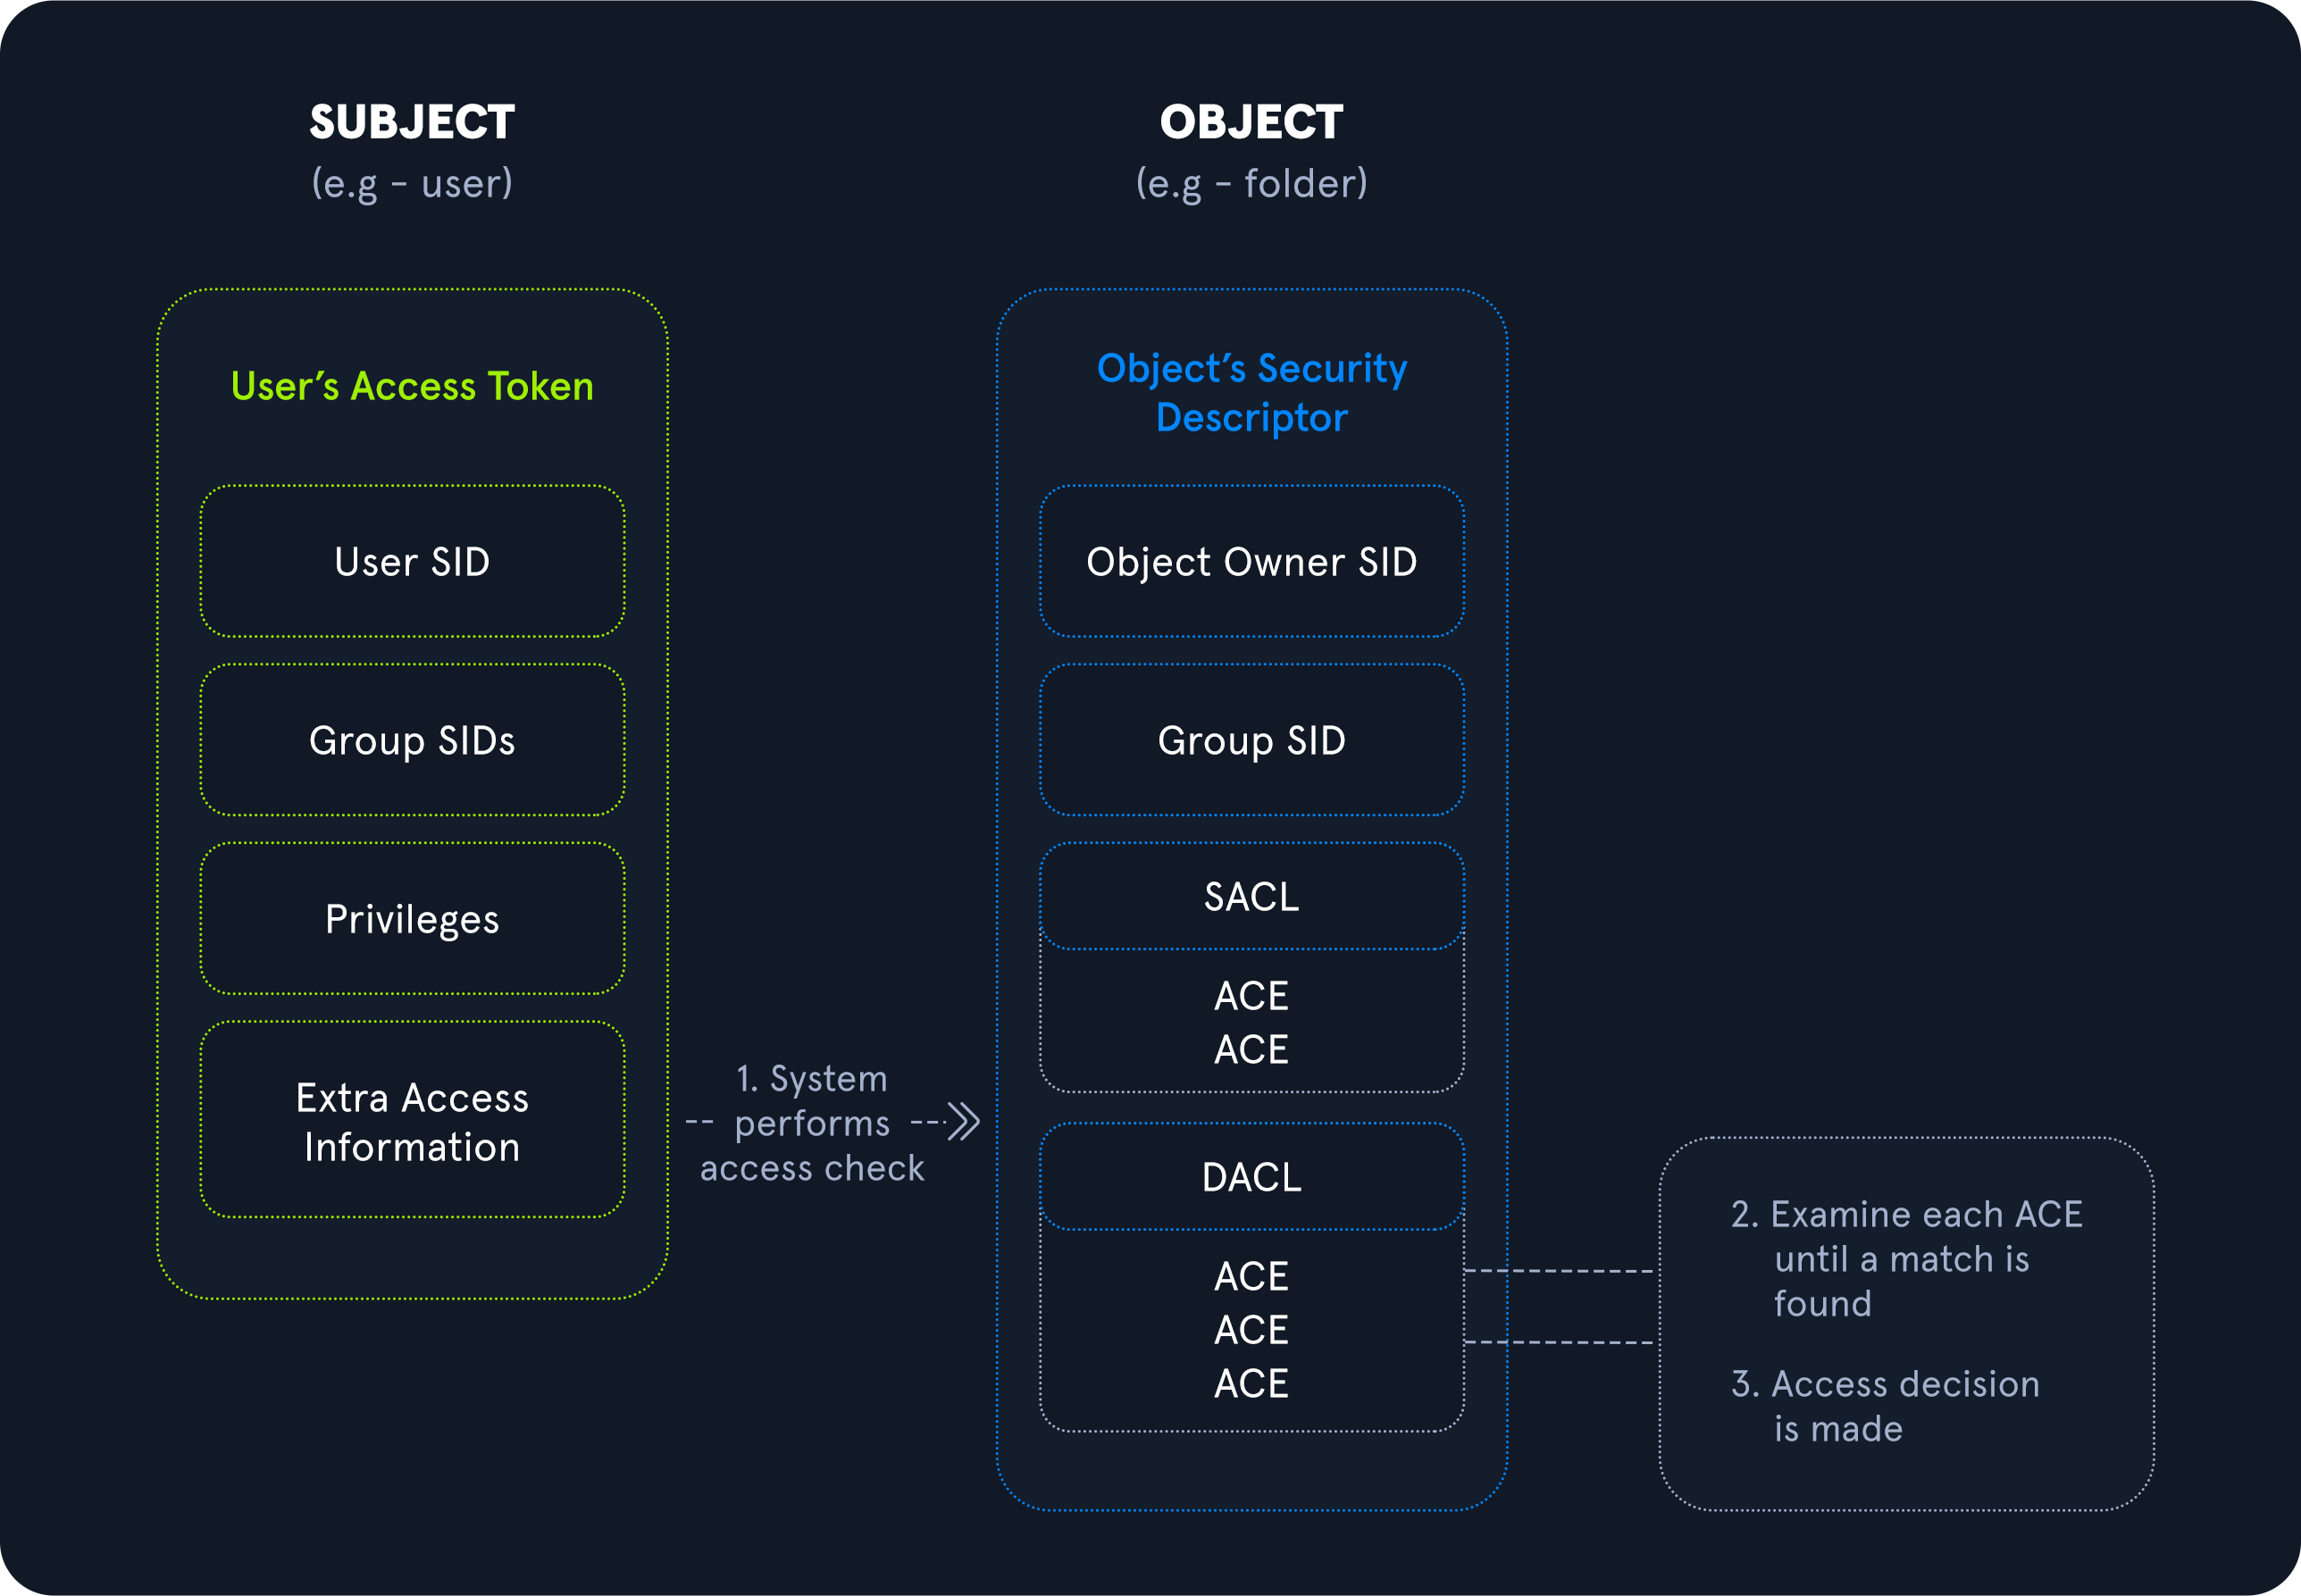
\includegraphics[width=\linewidth]{windows_knowledge/authorization/images/auth_process.png}
  \caption{Authorization process}
  \label{fig:authoriation process}
\end{figure}


Every object that can have a security descriptor (SD) is a
\href{https://docs.microsoft.com/en-us/windows/win32/secauthz/securable-objects}{securable object}
that may be protected by permissions. All named and several unnamed Windows
objects are securable and can have SDs, although this is not widely known.
There does not even exist a GUI for manipulating the SDs of many object types!
Have you ever tried to kill a system process in Task Manager and got the
message “Access denied”? This is due to the fact that this process’ SD does not
allow even administrators to kill the process. But it is, of course, possible,
as an administrator, to obtain the necessary permissions, provided a GUI or
some other tool is available.